\documentclass[dvipsnames]{beamer}

\usepackage[portuguese]{babel}
\usepackage{graphicx}
\usepackage{caption}
\usepackage{ragged2e}
\usepackage{amsmath}
\usepackage{amssymb}

\usepackage{tikz}
\usetikzlibrary{positioning}

\usefonttheme{serif}
\beamertemplatenavigationsymbolsempty

\title{Autoencoders}
\author{Eduardo de Medeiros da Silveira}
\institute{Universidade Federal de Santa Maria}
\date{}

\begin{document}

\frame{\titlepage}

\begin{frame}{Representação Eficiente de Dados}

	\justifying

	Em 1970, William Chase and Herbert Simon fizeram um experimento com jogadores profissionais de xadrez, para estudar a relação entre memória, percepção e reconhecimento de padrões.

	\begin{itemize}
		\item Capazes de memorizar o tabuleiro em poucos segundos.
		\item Somente quando as peças estavam em posições naturais.
		\item O reconhecimento de padrões ajuda na memorização.
	\end{itemize}

\end{frame}

\begin{frame}{Representação Eficiente de Dados}

	\begin{figure}

		\centering

		\begin{tikzpicture}

			\node[inner sep=0, outer sep=0] (chess-left) at (-3.5,0) {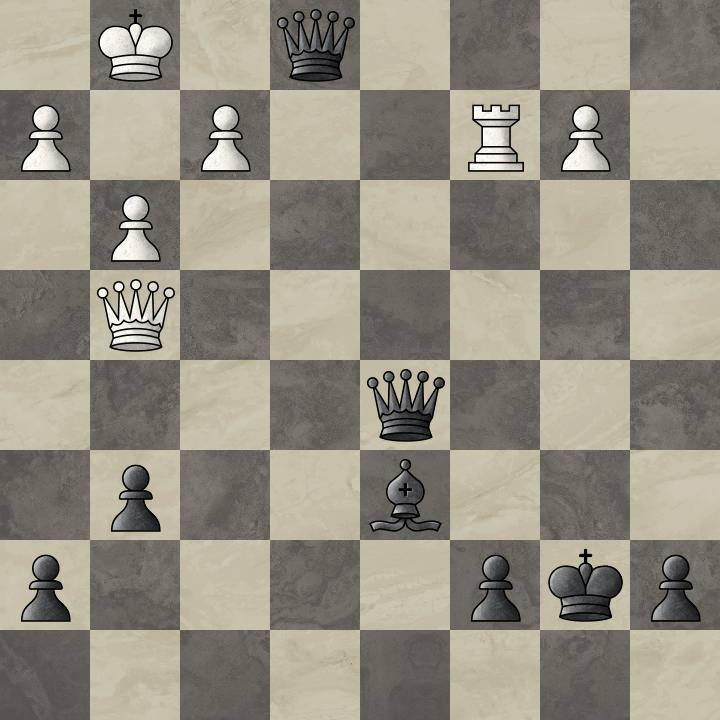
\includegraphics[width=.25\textwidth]{img/chess.jpeg}};
			\node[inner sep=0, outer sep=0, align=center] at (-3.5, 1.6) {Percepção};

			\node[inner sep=0] (abstract) at (0,0) {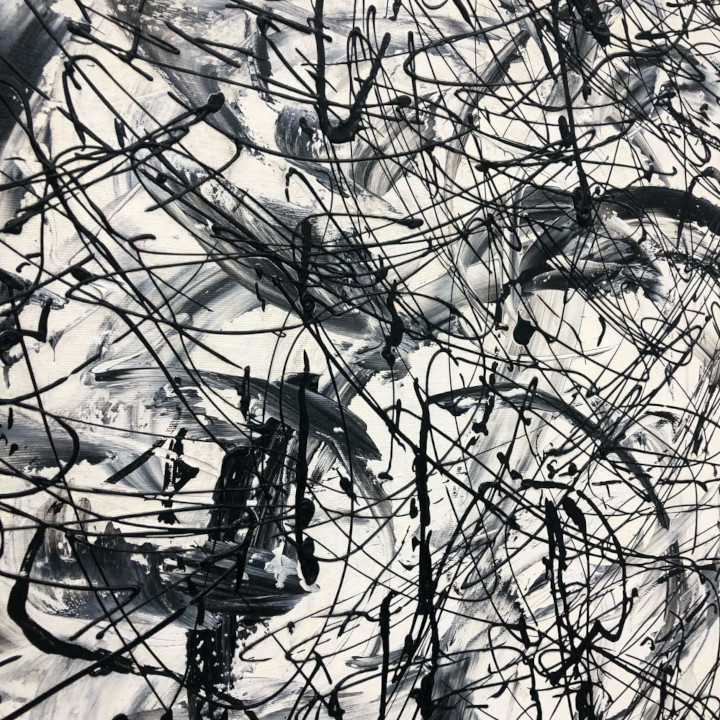
\includegraphics[width=.25\textwidth]{img/abstract.jpg}};
			\node[inner sep=0, outer sep=0, align=center] at (0, 1.6) {Memorização};

			\node[inner sep=0] (chess-right) at (3.5,0) {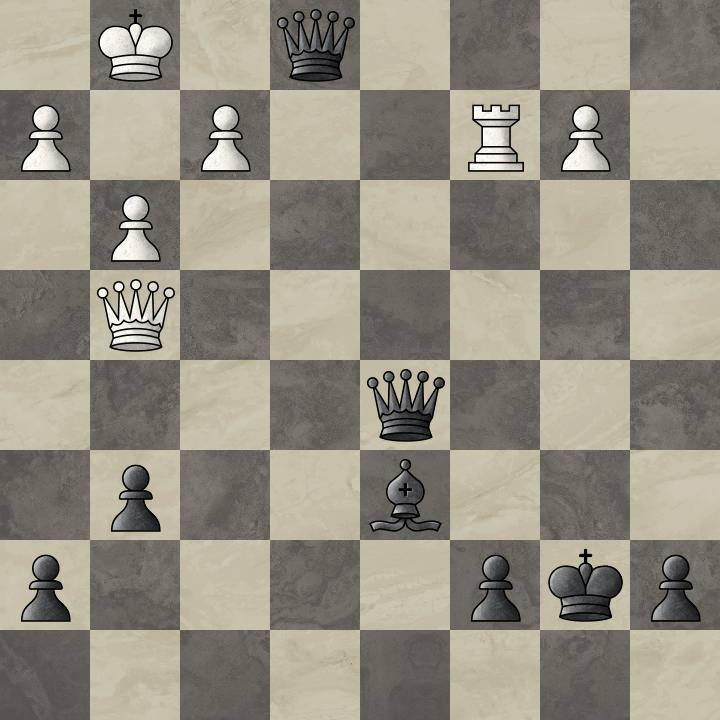
\includegraphics[width=.25\textwidth]{img/chess.jpeg}};
			\node[inner sep=0, outer sep=0, align=center] at (3.5, 1.6) {Recordação};

			\draw[->, thick] (chess-left.east) -- (abstract.west) node[midway, above] {};
			\draw[->, thick] (abstract.east) -- (chess-right.west) node[midway, above] {};

		\end{tikzpicture}

		\caption{Etapas do experimento da memória no xadrez.}

	\end{figure}

\end{frame}

\begin{frame}{Manifold Hypothesis}

	\begin{itemize}
		\item Conjuntos de dados com várias dimensões existem em \emph{manifolds} de menor dimensão.
	\end{itemize}

	\begin{figure}
		\centering
		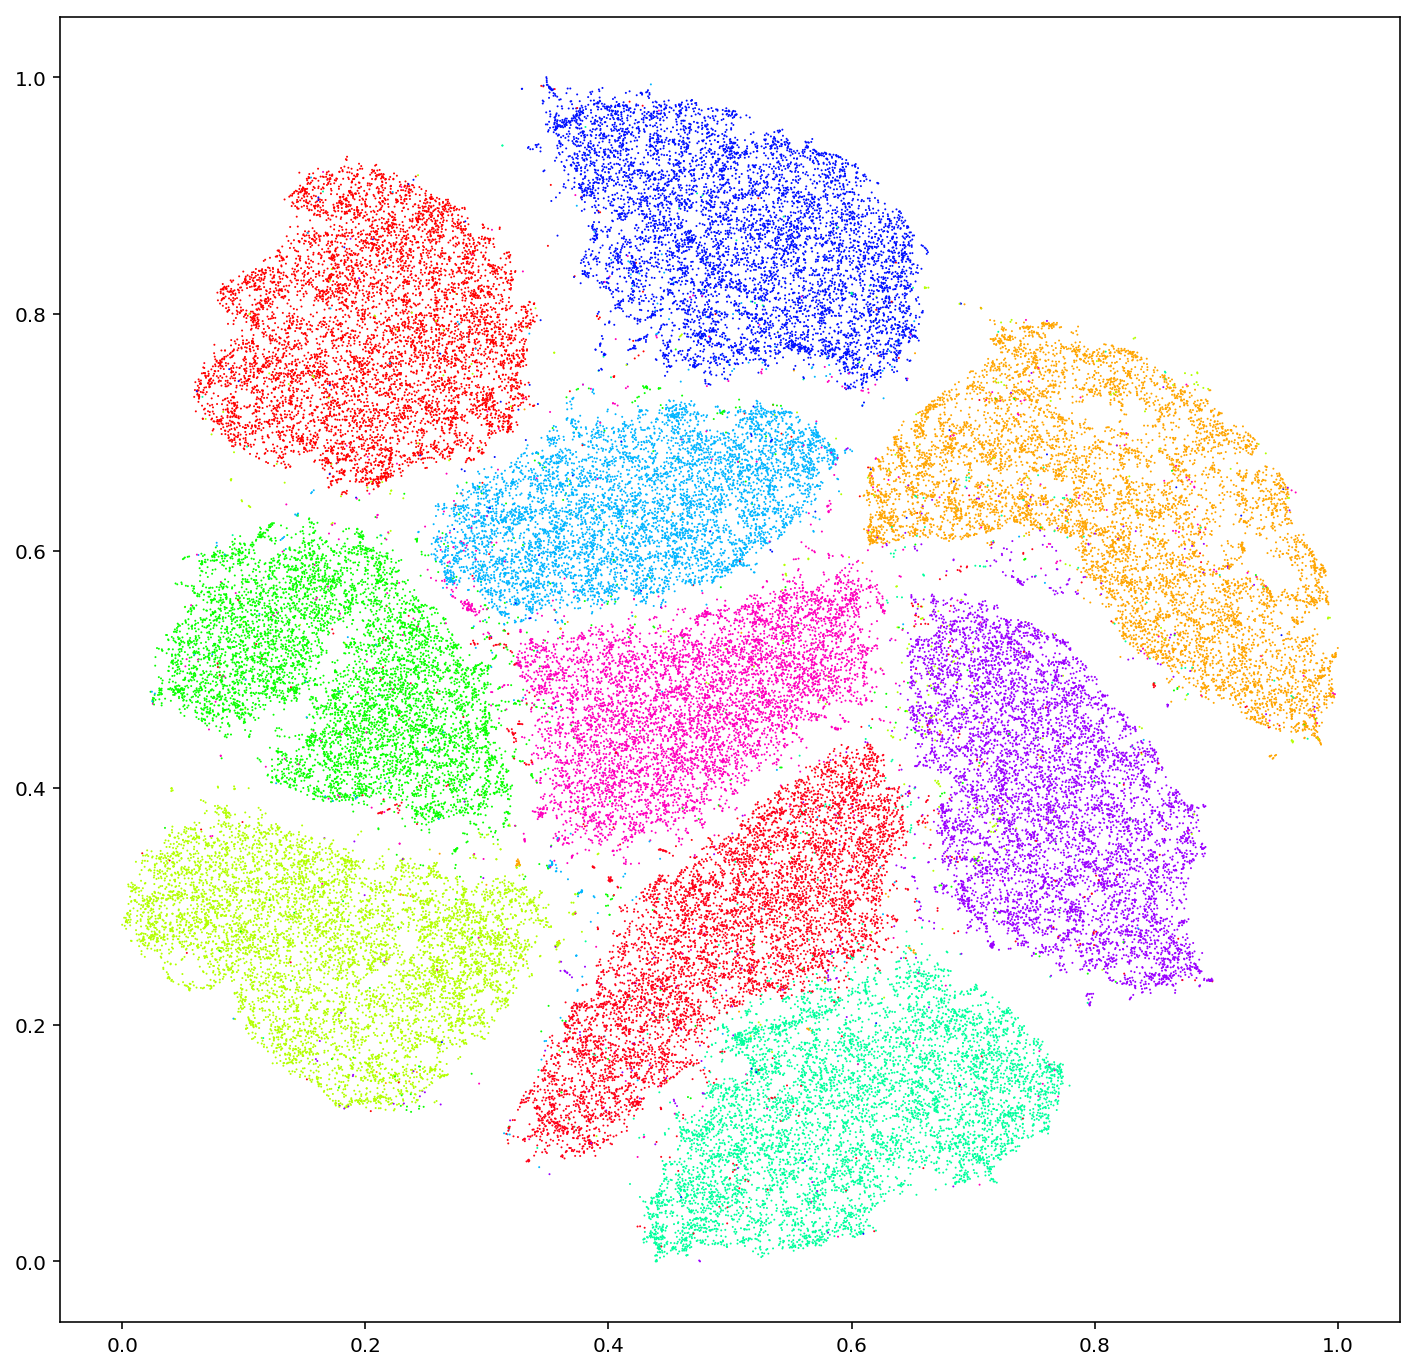
\includegraphics[scale=0.2]{img/tsne-mnist.png}
        \caption{Aplicação da técnica T-SNE ao MNIST.}
	\end{figure}

\end{frame}

\begin{frame}{Autoencoder}

	\justifying

	Um \emph{autoencoder} é uma rede neural que \textbf{tenta} aprender a função identidade.

	\begin{figure}

		\centering

		\begin{tikzpicture}[
				roundnode/.style={circle, draw=black, minimum size=10mm}
			]

			\node[roundnode] (hidden) {$\boldsymbol{h}$};
			\node[roundnode] (input) [below left=of hidden] {$\boldsymbol{x}$};
			\node[roundnode] (output) [below right= of hidden] {$\boldsymbol{x'}$};

			\draw[->] (input.north east) -- node[pos=0.35, above] {$f$} (hidden.south west);
			\draw[->] (hidden.south east) -- node[pos=0.65, above] {$g$} (output.north west);

		\end{tikzpicture}

		\caption{
			\justifying
			Esquema geral de um \emph{autoencoder}, que mapeia uma entrada $\boldsymbol{x}$ para uma saída $\boldsymbol{x'}$, através de uma representação interna $\boldsymbol{h}$.
			O \emph{autoencoder} é composto por um codificador $f$ e um decodificador $g$.
		}

	\end{figure}

\end{frame}

\begin{frame}{Autoencoder}

	Algumas características:

	\begin{itemize}
		\item Aprendizado não-supervisionado ou auto-supervisionado.
		\item A saída não importa.
		\item A representação latente $\boldsymbol{h}$ importa.
		\item Restrições.
	\end{itemize}

\end{frame}

\begin{frame}{Autoencoder}

	Algumas características:

	\begin{itemize}
		\item Mesmo número de neurônios na entrada e na saída.
		\item Geralmente é simétrico.
		\item \emph{Stacked} ou \emph{deep autoencoders}.
		\item Nem sempre $\boldsymbol{h}$ vai capturar informações importantes.
	\end{itemize}

	\begin{figure}

		\centering

		\begin{tikzpicture}[
				roundnode/.style={circle, draw=black, minimum size=2.5mm}
			]

			\def \dy {0.5}
			\def \dx {1}

			\foreach \i in {1, ..., 8} {
					\node[roundnode] (x-\i) at (0 * \dx, 0 + \i * \dy) {};
				}

			\foreach \i in {1, ..., 4} {
					\node[roundnode] (y-\i) at (1 * \dx, 1 + \i * \dy) {};
				}

			\foreach \i in {1, ..., 2} {
					\node[roundnode] (z-\i) at (2 * \dx, 1.5 + \i * \dy) {};
				}

			\foreach \i in {1, ..., 4} {
					\node[roundnode] (y'-\i) at (3 * \dx, 1 + \i * \dy) {};
				}

			\foreach \i in {1, ..., 8} {
					\node[roundnode] (x'-\i) at (4 * \dx, 0 + \i * \dy) {};
				}

			\foreach \i in {1, ..., 8} {
					\foreach \j in {1, ..., 4} {
							\draw[color=gray] (x-\i) -- (y-\j);
						}
				}

			\foreach \i in {1, ..., 8} {
					\foreach \j in {1, ..., 4} {
							\draw[color=gray] (x'-\i) -- (y'-\j);
						}
				}

			\foreach \i in {1, ..., 4} {
					\foreach \j in {1, ..., 2} {
							\draw[color=gray] (y-\i) -- (z-\j);
						}
				}

			\foreach \i in {1, ..., 4} {
					\foreach \j in {1, ..., 2} {
							\draw[color=gray] (y'-\i) -- (z-\j);
						}
				}

		\end{tikzpicture}

		\caption{Exemplo de um autoencoder.}

	\end{figure}

\end{frame}

\begin{frame}{Undercomplete Autoencoder}

	\justifying

	\begin{itemize}
		\item A dimensão de $\boldsymbol{h}$ é menor do que a dimensão de $\boldsymbol{x}$.
		\item Minimiza-se $L$, que calcula a dissimilaridade de $\boldsymbol{x}$ e $\boldsymbol{x'}$.
	\end{itemize}

	\begin{equation*}
		L(\boldsymbol{x}, \boldsymbol{x'}) = L(\boldsymbol{x}, g(f(\boldsymbol{x})))
	\end{equation*}

\end{frame}

\begin{frame}{Pré-treino não-supervisionado}

	\justifying

	\begin{itemize}
		\item Queremos treinar um modelo supervisionado.
		\item Temos poucas observações rotuladas.
		\item Podemos treinar um \emph{autoencoder} e reutilizar o \emph{encoder}.
		\item Congelamento dos parâmetros.
	\end{itemize}

	\begin{figure}

		\centering

		\begin{tikzpicture}[
				roundnode/.style={draw=black, thick, rounded corners}
			]

			\def \dx {5};

			\node[roundnode, minimum width=32mm] (output) at (0, 4) {Saída};
			\node[roundnode, minimum width=16mm] (h3) at (0, 3) {$h_3$};
			\node[roundnode, minimum width=8mm] (h2) at (0, 2) {$h_2$};
			\node[roundnode, minimum width=16mm] (h1) at (0, 1) {$h_1$};
			\node[roundnode, minimum width=32mm] (input) at (0, 0) {Entrada};

			\node[roundnode] (output') at (\dx, 4) {Saída};
			\node[fill=black, minimum width=8mm, minimum height=8mm] (h3') at (\dx, 3.05) {};
			\node[roundnode, RoyalBlue, minimum width=8mm] (h2') at (\dx, 2) {$h_2$};
			\node[roundnode, RoyalBlue, minimum width=16mm] (h1') at (\dx, 1) {$h_1$};
			\node[roundnode, minimum width=32mm] (input') at (\dx, 0) {Entrada};

			\draw[->, thick] (input) -- (h1);
			\draw[->, thick] (h1) -- (h2);
			\draw[->, thick] (h2) -- (h3);
			\draw[->, thick] (h3) -- (output);

			\draw[->, RoyalBlue, thick] (input') -- (h1');
			\draw[->, RoyalBlue, thick] (h1') -- (h2');
			\draw[->, thick] (h2') -- (h3');
			\draw[->, thick] (h3') -- (output');

			\draw[->, dashed, RoyalBlue, thick] (h1) -- (h1');
			\draw[->, dashed, RoyalBlue, thick] (h2) -- (h2');

		\end{tikzpicture}

		\caption{Aproveitamento da função de \emph{encoding} em outra rede neural.}

	\end{figure}

\end{frame}

\begin{frame}{Enlace de parâmetros}

	\begin{itemize}
		\item Se o \emph{autoencoder} for simétrico, podemos criar um enlace entre os parâmetros do \emph{encoder} e \emph{decoder}.
		\item Reduzimos pela metade o número de parâmetros.
		\item O vetor de viés é mantido.
	\end{itemize}

	\begin{figure}

		\centering

		\begin{tikzpicture}[
				roundnode/.style={draw=black, thick, rounded corners}
			]

			\def \dx {5};

			\node[roundnode, minimum width=32mm] (output) at (0, 4) {Saída};
			\node[roundnode, minimum width=16mm] (h3) at (0, 3) {$h_3$};
			\node[roundnode, minimum width=8mm] (h2) at (0, 2) {$h_2$};
			\node[roundnode, minimum width=16mm] (h1) at (0, 1) {$h_1$};
			\node[roundnode, minimum width=32mm] (input) at (0, 0) {Entrada};

			\draw[->, RoyalBlue, thick] (input) -- node[midway, left] {\small$\boldsymbol{W}_1$} (h1);
			\draw[->, Green, thick] (h1) -- node[midway, right] {\small$\boldsymbol{W}_2$} (h2);
			\draw[->, Green, thick] (h2) -- node[midway, right] {\small$\boldsymbol{W}_3$} (h3);
			\draw[->, RoyalBlue, thick] (h3) -- node[midway, left] {\small$\boldsymbol{W}_4$} (output);

			\draw[RoyalBlue, dashed, thick] (0, 0.5) .. controls (3, 0.5) and (3, 3.5) .. node[midway, right] {$\boldsymbol{W}_4 = \boldsymbol{W}_1^\top$} (0, 3.5);
			\draw[Green, dashed, thick] (0, 1.5) .. controls (-1, 1.5) and (-1, 2.5) .. node[midway, left] {$\boldsymbol{W}_3 = \boldsymbol{W}_2^\top$} (0, 2.5);


		\end{tikzpicture}

		\caption{Enlace dos parâmetros de um \emph{encoder} e um \emph{decoder}.}

	\end{figure}

\end{frame}

\begin{frame}{Treinamento por Camadas}

	Em vez de treinar todo o \emph{autoencoder}, podemos dividir o treino por camadas.

	\begin{figure}

		\centering

		\begin{tikzpicture}[
				roundnode/.style={draw=black, thick, rounded corners}
			]

			\node[roundnode, minimum width=32mm, Green] (output1) at (0, 4) {Saída};
			\node[roundnode, minimum width=16mm, RoyalBlue] (h1) at (0, 1) {$h_1$};
			\node[roundnode, minimum width=32mm] (input1) at (0, 0) {Entrada};

			\node[roundnode, minimum width=16mm, Purple] (output2) at (3, 3) {Saída};
			\node[roundnode, minimum width=8mm, Orange] (h2) at (3, 2) {$h_2$};
			\node[roundnode, minimum width=16mm] (input2) at (3, 1) {Entrada};

			\node[roundnode, minimum width=32mm, Green] (output3) at (6, 4) {Saída};
			\node[roundnode, minimum width=16mm, Purple] (h3) at (6, 3) {$h_3$};
			\node[roundnode, minimum width=8mm, Orange] (h2') at (6, 2) {$h_2$};
			\node[roundnode, minimum width=16mm, RoyalBlue] (h1') at (6, 1) {$h_1$};
			\node[roundnode, minimum width=32mm] (input3) at (6, 0) {Entrada};

			\draw[->, thick, RoyalBlue] (input1) -- (h1);
			\draw[->, thick, Green] (h1) -- (output1);

			\draw[->, thick, Orange] (input2) -- (h2);
			\draw[->, thick, Purple] (h2) -- (output2);

			\draw[->, thick, RoyalBlue] (input3) -- (h1');
			\draw[->, thick, Orange] (h1') -- (h2');
			\draw[->, thick, Purple] (h2') -- (h3);
			\draw[->, thick, Green] (h3) -- (output3);

			\draw[->, dashed, thick, RoyalBlue] (h1) -- (1.8, 1) -- (1.8, 0.4) -- (4.2, 0.4) -- (4.2, 1) -- (h1');
			\draw[->, dashed, thick, Orange] (h2) -- (h2');
			\draw[->, dashed, thick, Purple] (output2) -- (h3);
			\draw[->, dashed, thick, Green] (output1) -- (output3);

		\end{tikzpicture}

		\caption{Treinamento por camadas de um \emph{autoencoder}. Primeiramente, treinamos as camadas $h_1$ e Saída. Depois, treinamos $h_2$ e $h_3$.}

	\end{figure}

\end{frame}

\begin{frame}{Convolutional Autoencoders}

	\begin{itemize}
		\item Camadas convolucionais em vez de camadas densas.
		\item Principalmente para imagens.
		\item O \emph{encoder} faz a compressão da imagem, enquanto o \emph{decoder} faz a decompressão (camadas transpostas).
	\end{itemize}

    \begin{figure}
        \centering
        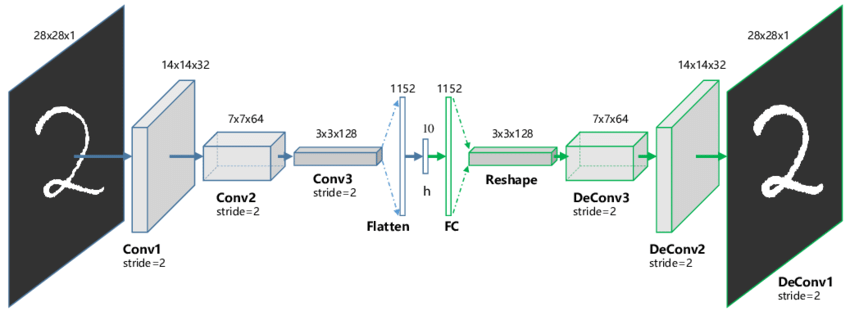
\includegraphics[scale=0.33]{img/conv-autoencoder.png} 
        \caption{Exemplo de um autoencoder convolucional.}
    \end{figure}

\end{frame}

\begin{frame}{Overcomplete Autoencoders}

	\begin{itemize}
		\item A representação latente $\boldsymbol{h}$ tem dimensão maior ou igual à da entrada.
	\end{itemize}

	\begin{figure}

		\centering

		\begin{tikzpicture}[
				roundnode/.style={circle, draw=black, minimum size=2.5mm}
			]

			\def \dy {0.5}
			\def \dx {1}

			\foreach \i in {1, ..., 4} {
					\node[roundnode] (x-\i) at (0 * \dx, 1 + \i * \dy) {};
				}

			\foreach \i in {1, ..., 8} {
					\node[roundnode] (y-\i) at (1 * \dx, 0 + \i * \dy) {};
				}

			\foreach \i in {1, ..., 4} {
					\node[roundnode] (x'-\i) at (2 * \dx, 1 + \i * \dy) {};
				}

			\foreach \i in {1, ..., 4} {
					\foreach \j in {1, ..., 8} {
							\draw[color=gray] (x-\i) -- (y-\j);
						}
				}

			\foreach \i in {1, ..., 4} {
					\foreach \j in {1, ..., 8} {
							\draw[color=gray] (x'-\i) -- (y-\j);
						}
				}

		\end{tikzpicture}

		\caption{Exemplo de um autoencoder overcomplete.}

	\end{figure}

\end{frame}

\begin{frame}{Denoising Autoencoders}

	\begin{itemize}
		\item Adição de ruído na entrada (Gaussiano ou Dropout).
		\item Treinamento para recuperar os dados originais.
	\end{itemize}

	$$L(\boldsymbol{x}, g(f(\tilde{\boldsymbol{x}})))$$

	\begin{figure}

		\centering

		\begin{tikzpicture}[
				roundnode/.style={draw=black, thick, rounded corners}
			]

			\node[roundnode, minimum width=32mm] (output) at (0, 3) {Saída};
			\node[roundnode, minimum width=16mm] (h) at (0, 2) {$h$};
			\node[roundnode, fill=Red, text=White] (noise) at (0, 1) {Ruído};
			\node[roundnode, minimum width=32mm] (input) at (0, 0) {Entrada};

			\draw[->, thick] (input) -- (noise);
			\draw[->, thick] (noise) -- (h);
			\draw[->, thick] (h) -- (output);

		\end{tikzpicture}

		\caption{
			\justifying
			Esquema de um \emph{denoising autoencoder}. O ruído pode representar a adição de ruído Gaussiano aos dados ou uma camada de Dropout.
		}

	\end{figure}

\end{frame}

\begin{frame}{Sparse Autoencoders}

	\begin{itemize}
		\item A representação latente é penalizada por sua esparsidade.
		\item Escolhemos uma quantidade de neurônios que queremos ativados.
		\item Cada neurônio acaba representando uma característica específica.
	\end{itemize}

	$$L(\boldsymbol{x}, \boldsymbol{x'}) + \Omega(\boldsymbol{h}) = L(\boldsymbol{x}, g(f(\boldsymbol{x}))) + \Omega(\boldsymbol{h})$$

\end{frame}

\begin{frame}{Variational Autoencoders}
	\begin{itemize}
		\item São probabilísticos (a saída não é determinística).
		\item São generativos.
		\item O \emph{encoder} produz uma média $\boldsymbol{\mu}$ e desvio padrão $\boldsymbol{\sigma}$.
		\item A representação latente é amostrada de $\mathcal{N}(\mu_i, \sigma_i)$.
		\item O \emph{decoder} age sobre a representação amostrada.
	\end{itemize}
\end{frame}

\end{document}
